\section{Design and Implementation}

\subsection{Hardware Design}


\subsubsection{Waist}
The waist joint of the arm is mounted directly to the frame of Tiberius using an M12 bolt. The joint contains 3 bearings and is powered by a 2.5:1 ratio timing belt drive. The home position is at the maximum extent of the axis with the endstop mounted on the extrusion under the arm.

\begin{figure}[!htb]
\begin{center}
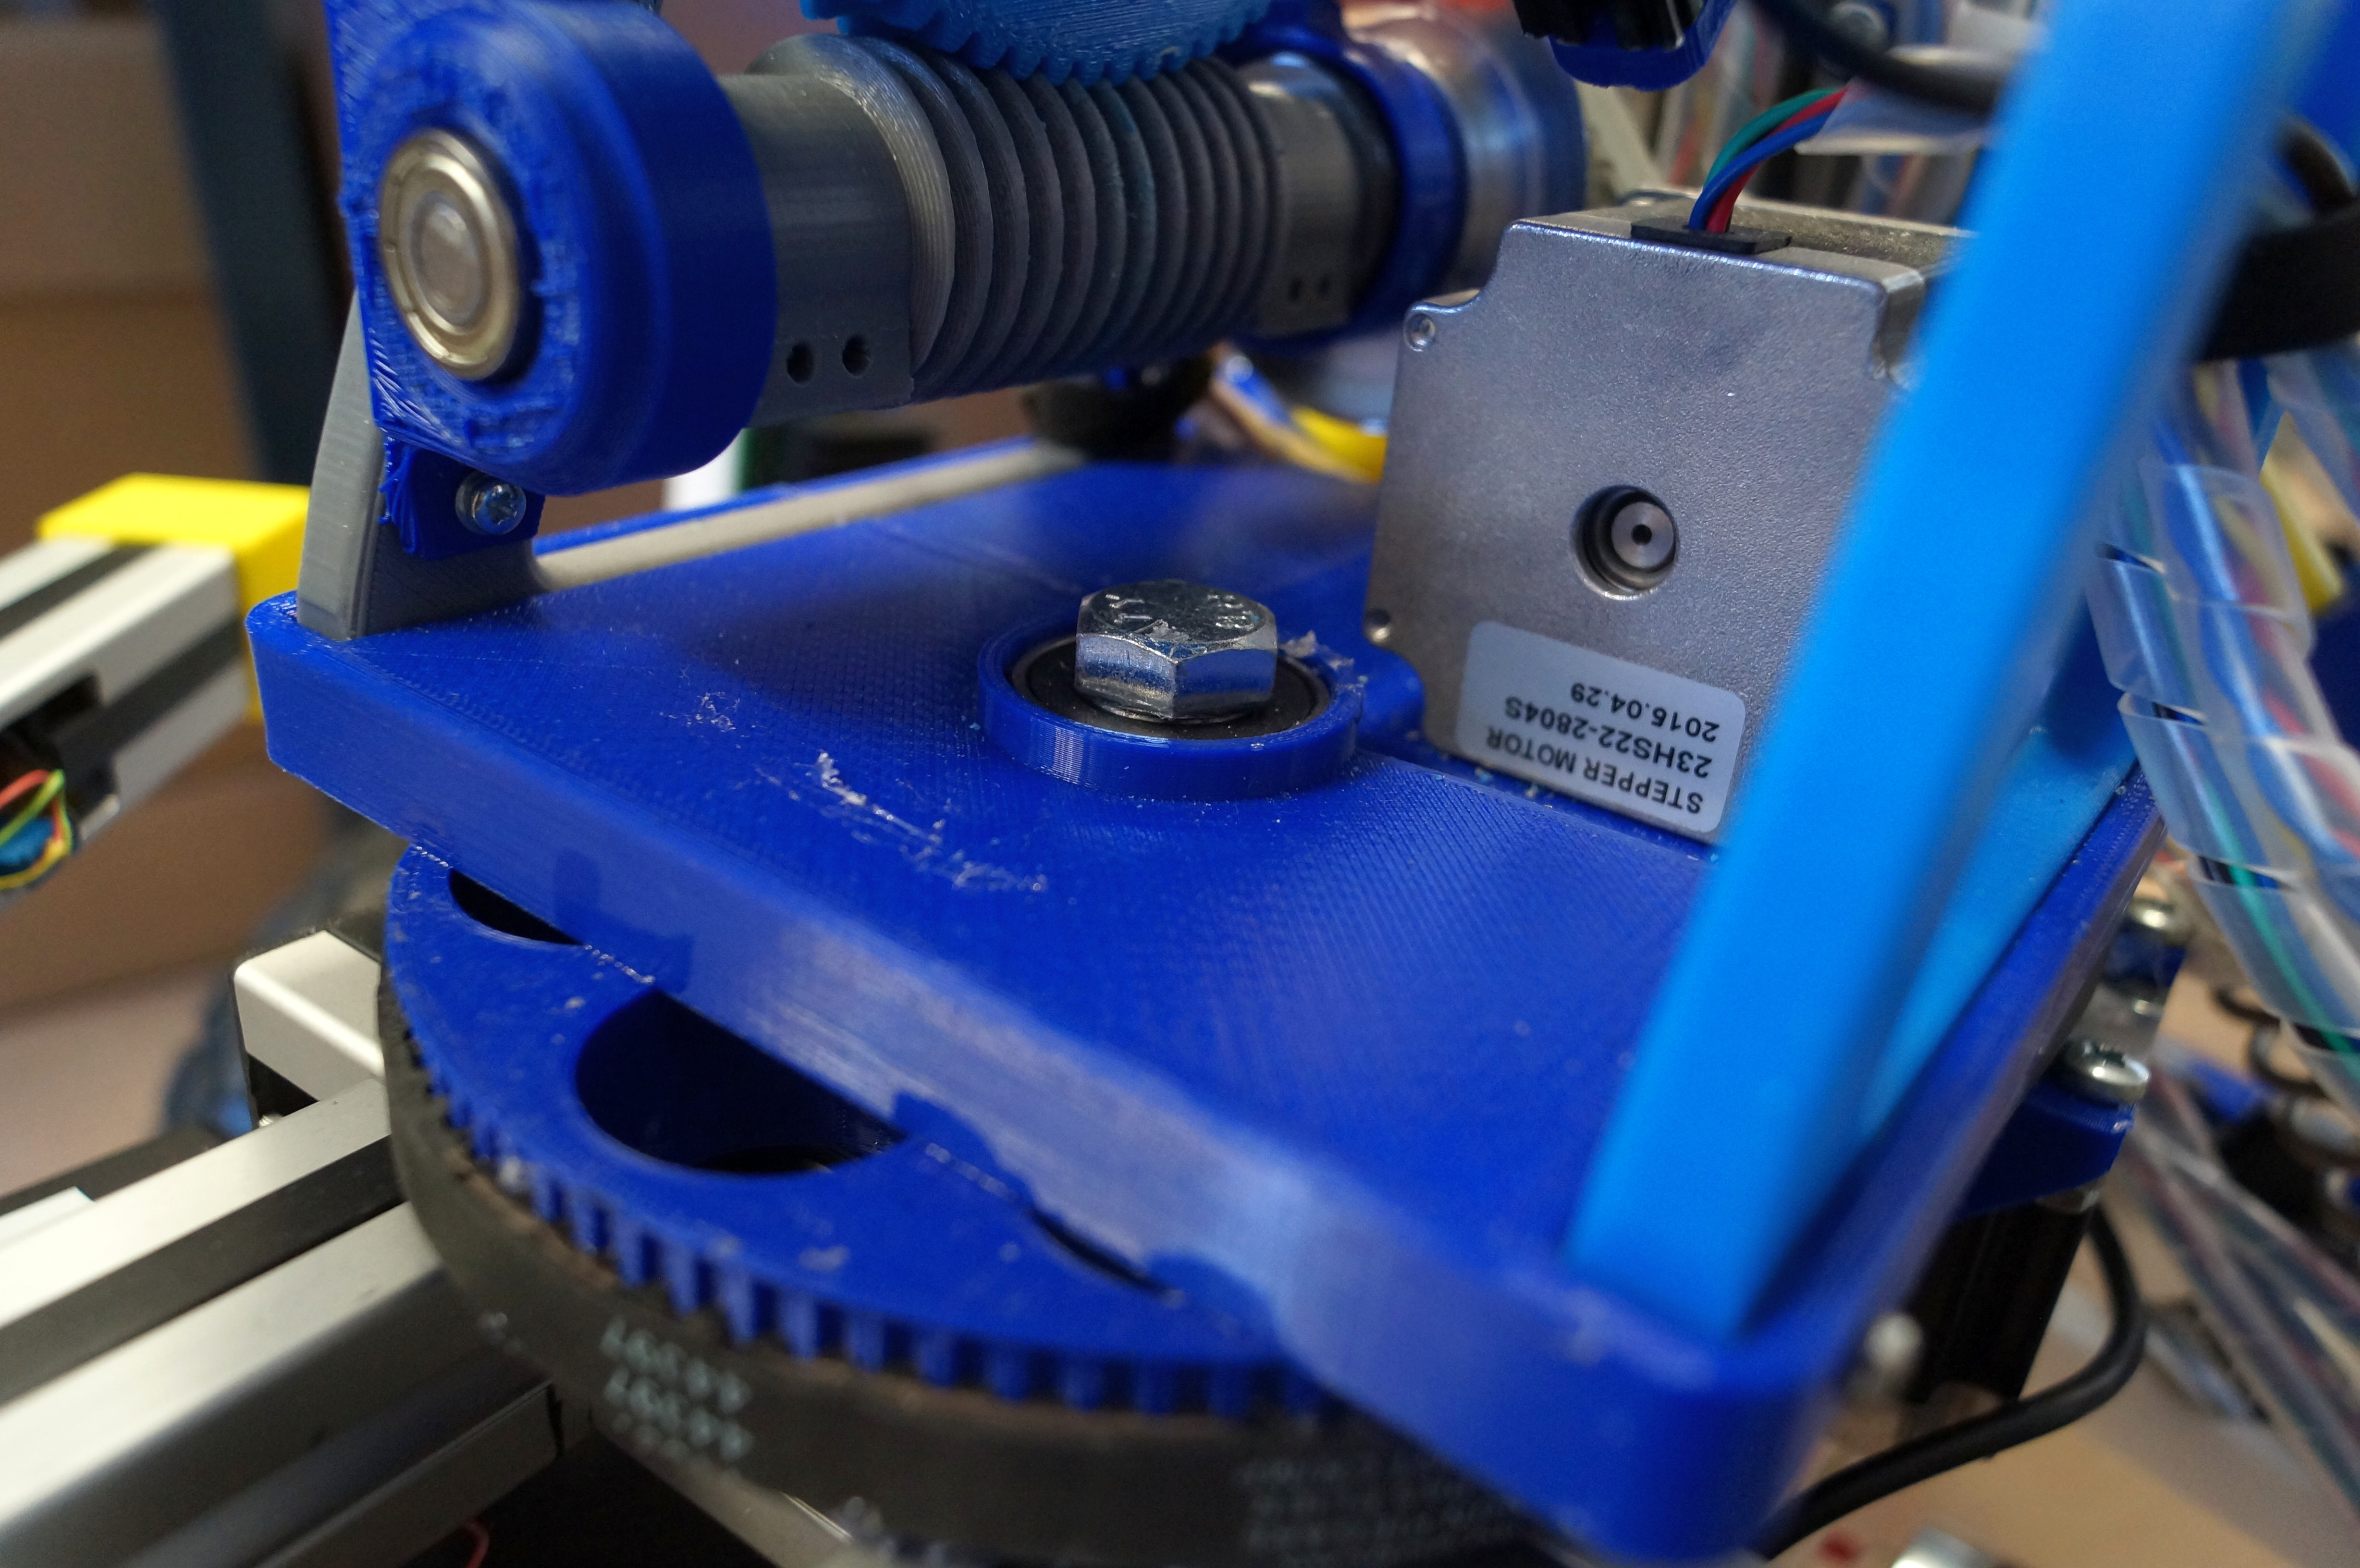
\includegraphics[width=10cm]{waist.jpg}
\end{center}
\caption{Waist Joint}
\label{fig:waist}
\end{figure}

\subsubsection{Shoulder}
The shoulder joint is raised up on an A-frame mounted to the waist by M3 bolts. A shaft runs through the centre of the joint with bearings on either end and held in place with collars. The joint is powered by a 160:1 worm drive which allows the arm to have a theoretical torque of 284Nm. Clearly this would be impossible to achieve unless the gears were made of metal, the arm was tested to 20Nm with no problem although the plastic gears are likely to be damaged if this value is exceeded. The reason for such a high designed torque was to reduce the torque required to turn the pulleys, which in turn reduces the power consumption of the arm. The extrusion slides into the holes in the joint and is held in place with a fixing plate and bolts. The worm gear is also mounted with 4 bearings in order to stop the plastic welding together from friction.

\begin{figure}[!htb]
\begin{center}
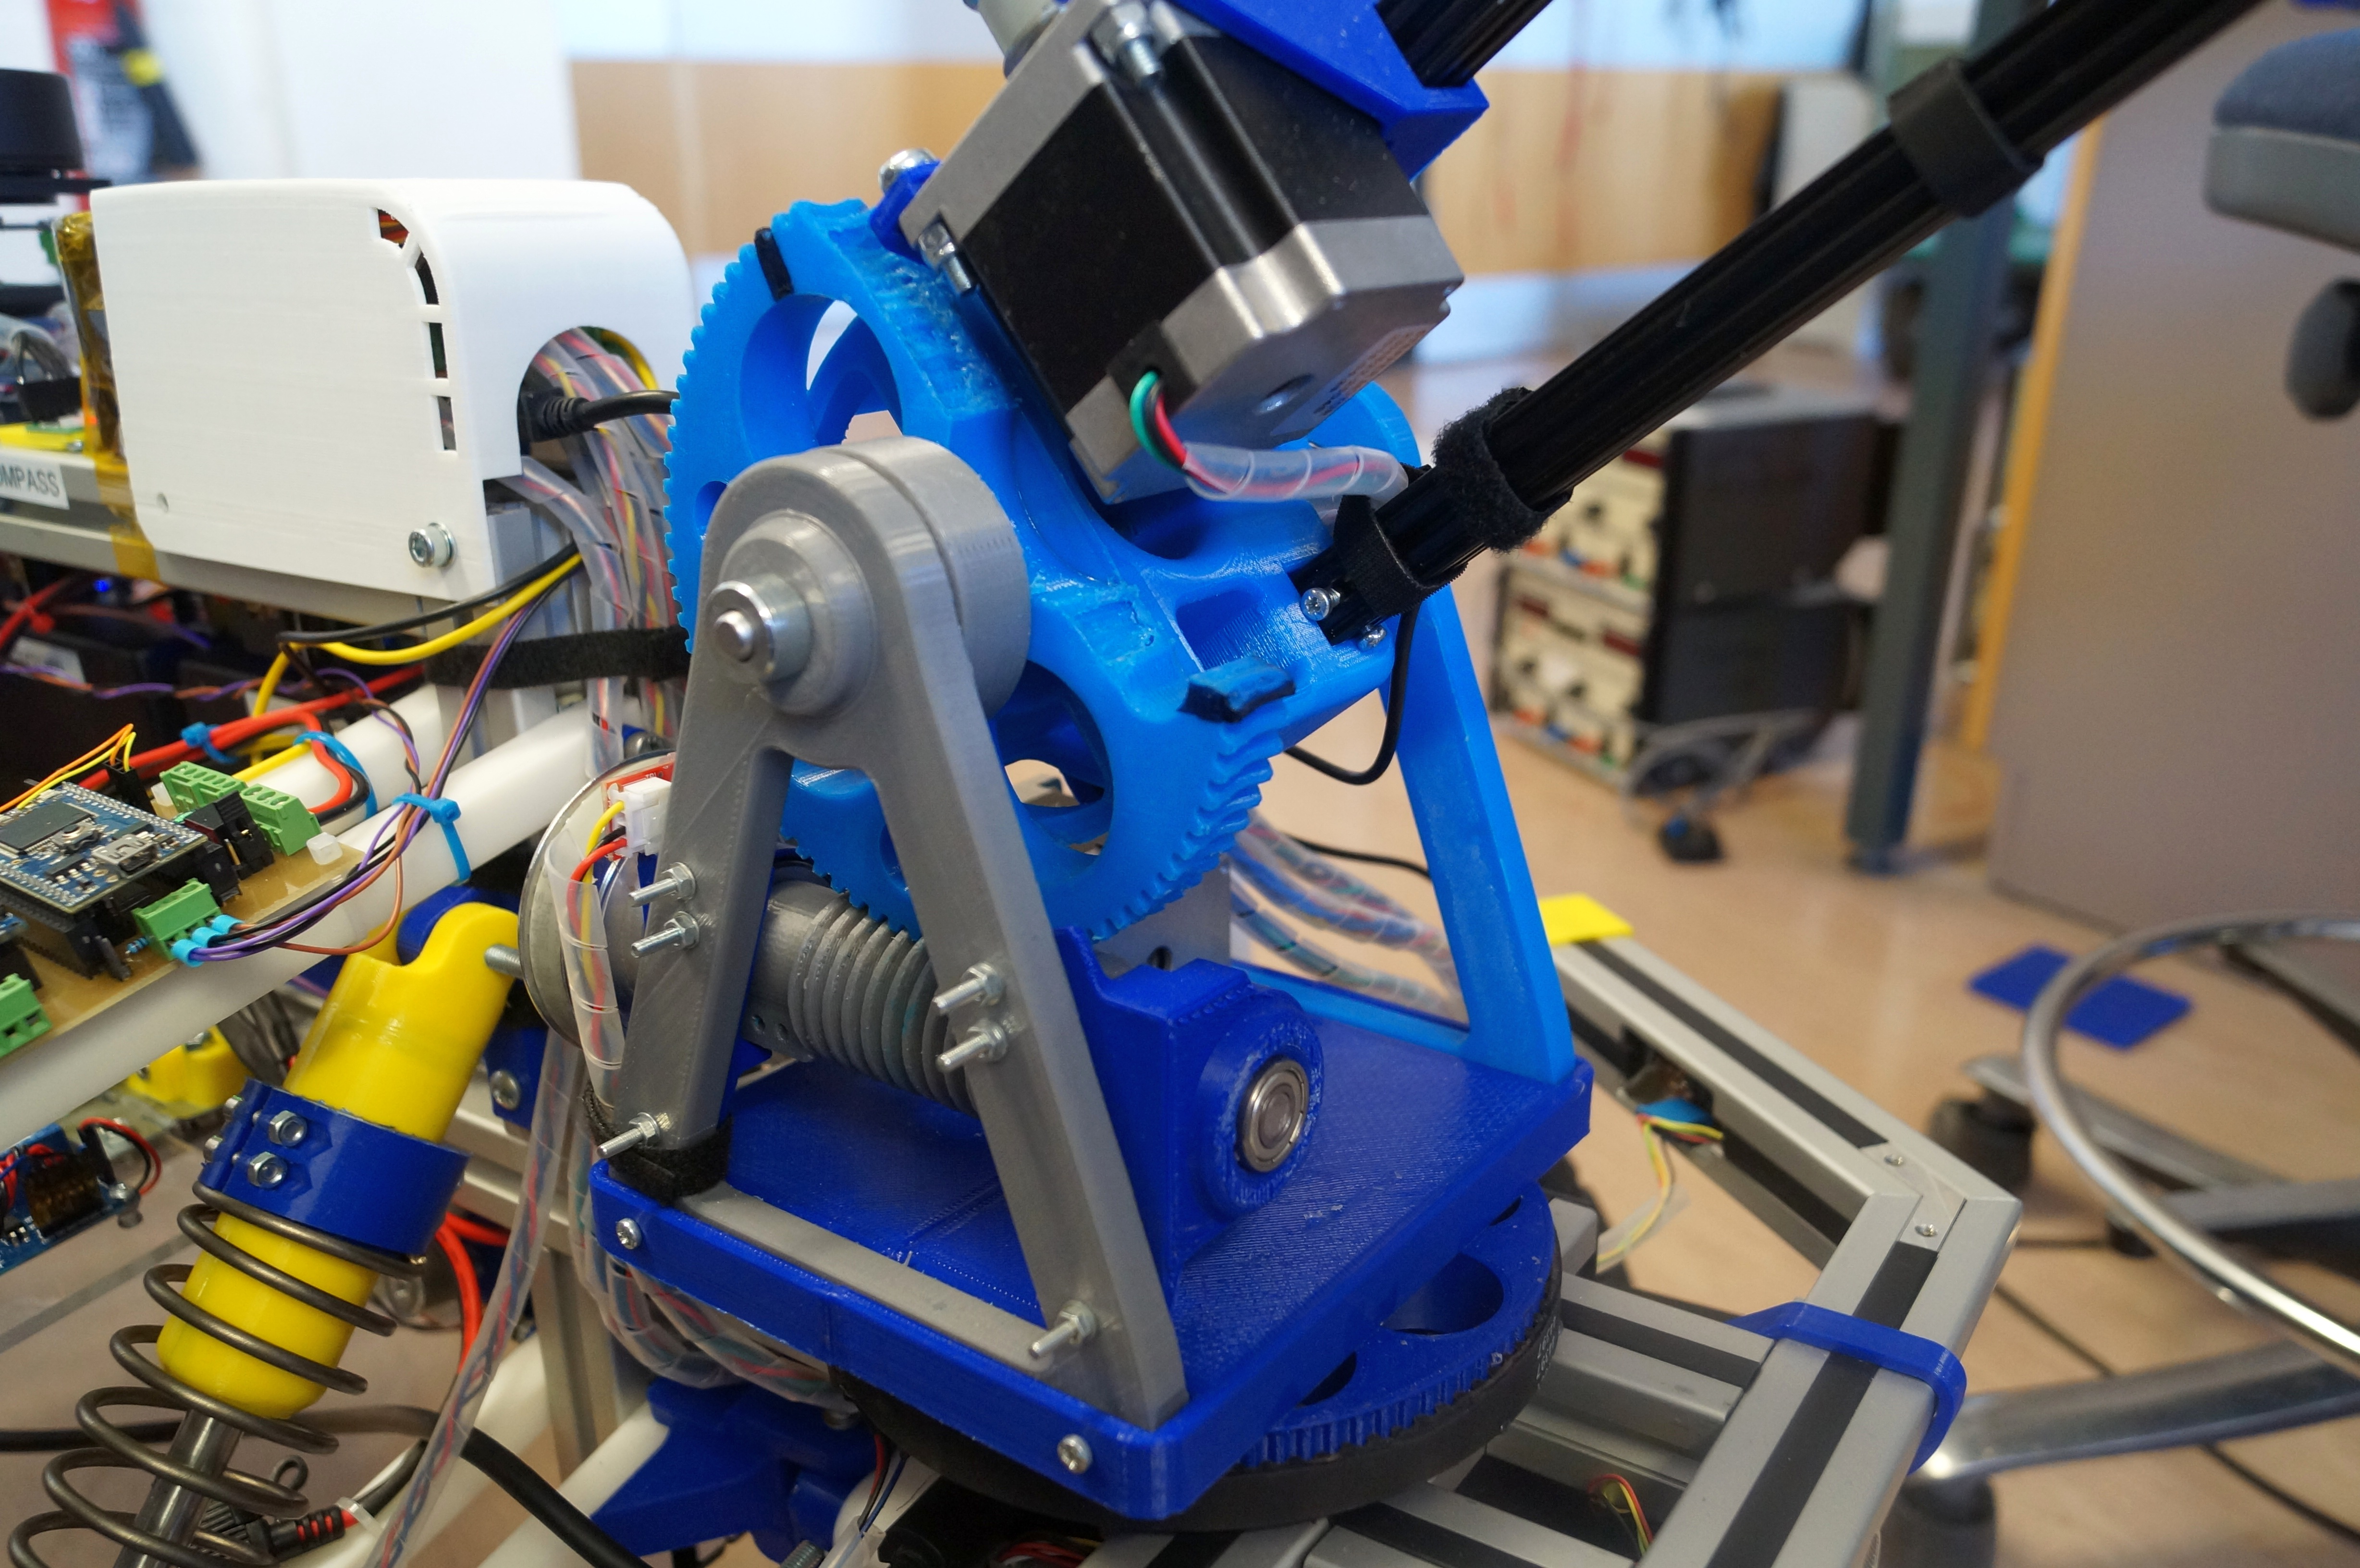
\includegraphics[width=10cm]{base.jpg}
\end{center}
\caption{Shoulder Joint}
\label{fig:shoulder}
\end{figure}

\subsubsection{Elbow}
The elbow joint is a condensed version of the shoulder, using an M8 bolt as the pivot point with 4 thrust bearings to reduce friction while keeping the joint tight. The worm drive is identical to the shoulder but the gear ratio is only 80:1 which is suitable since there will be less load on the joint than the shoulder. The worm is mounted in a similar fashion to the shoulder.

\begin{figure}[!htb]
\begin{center}
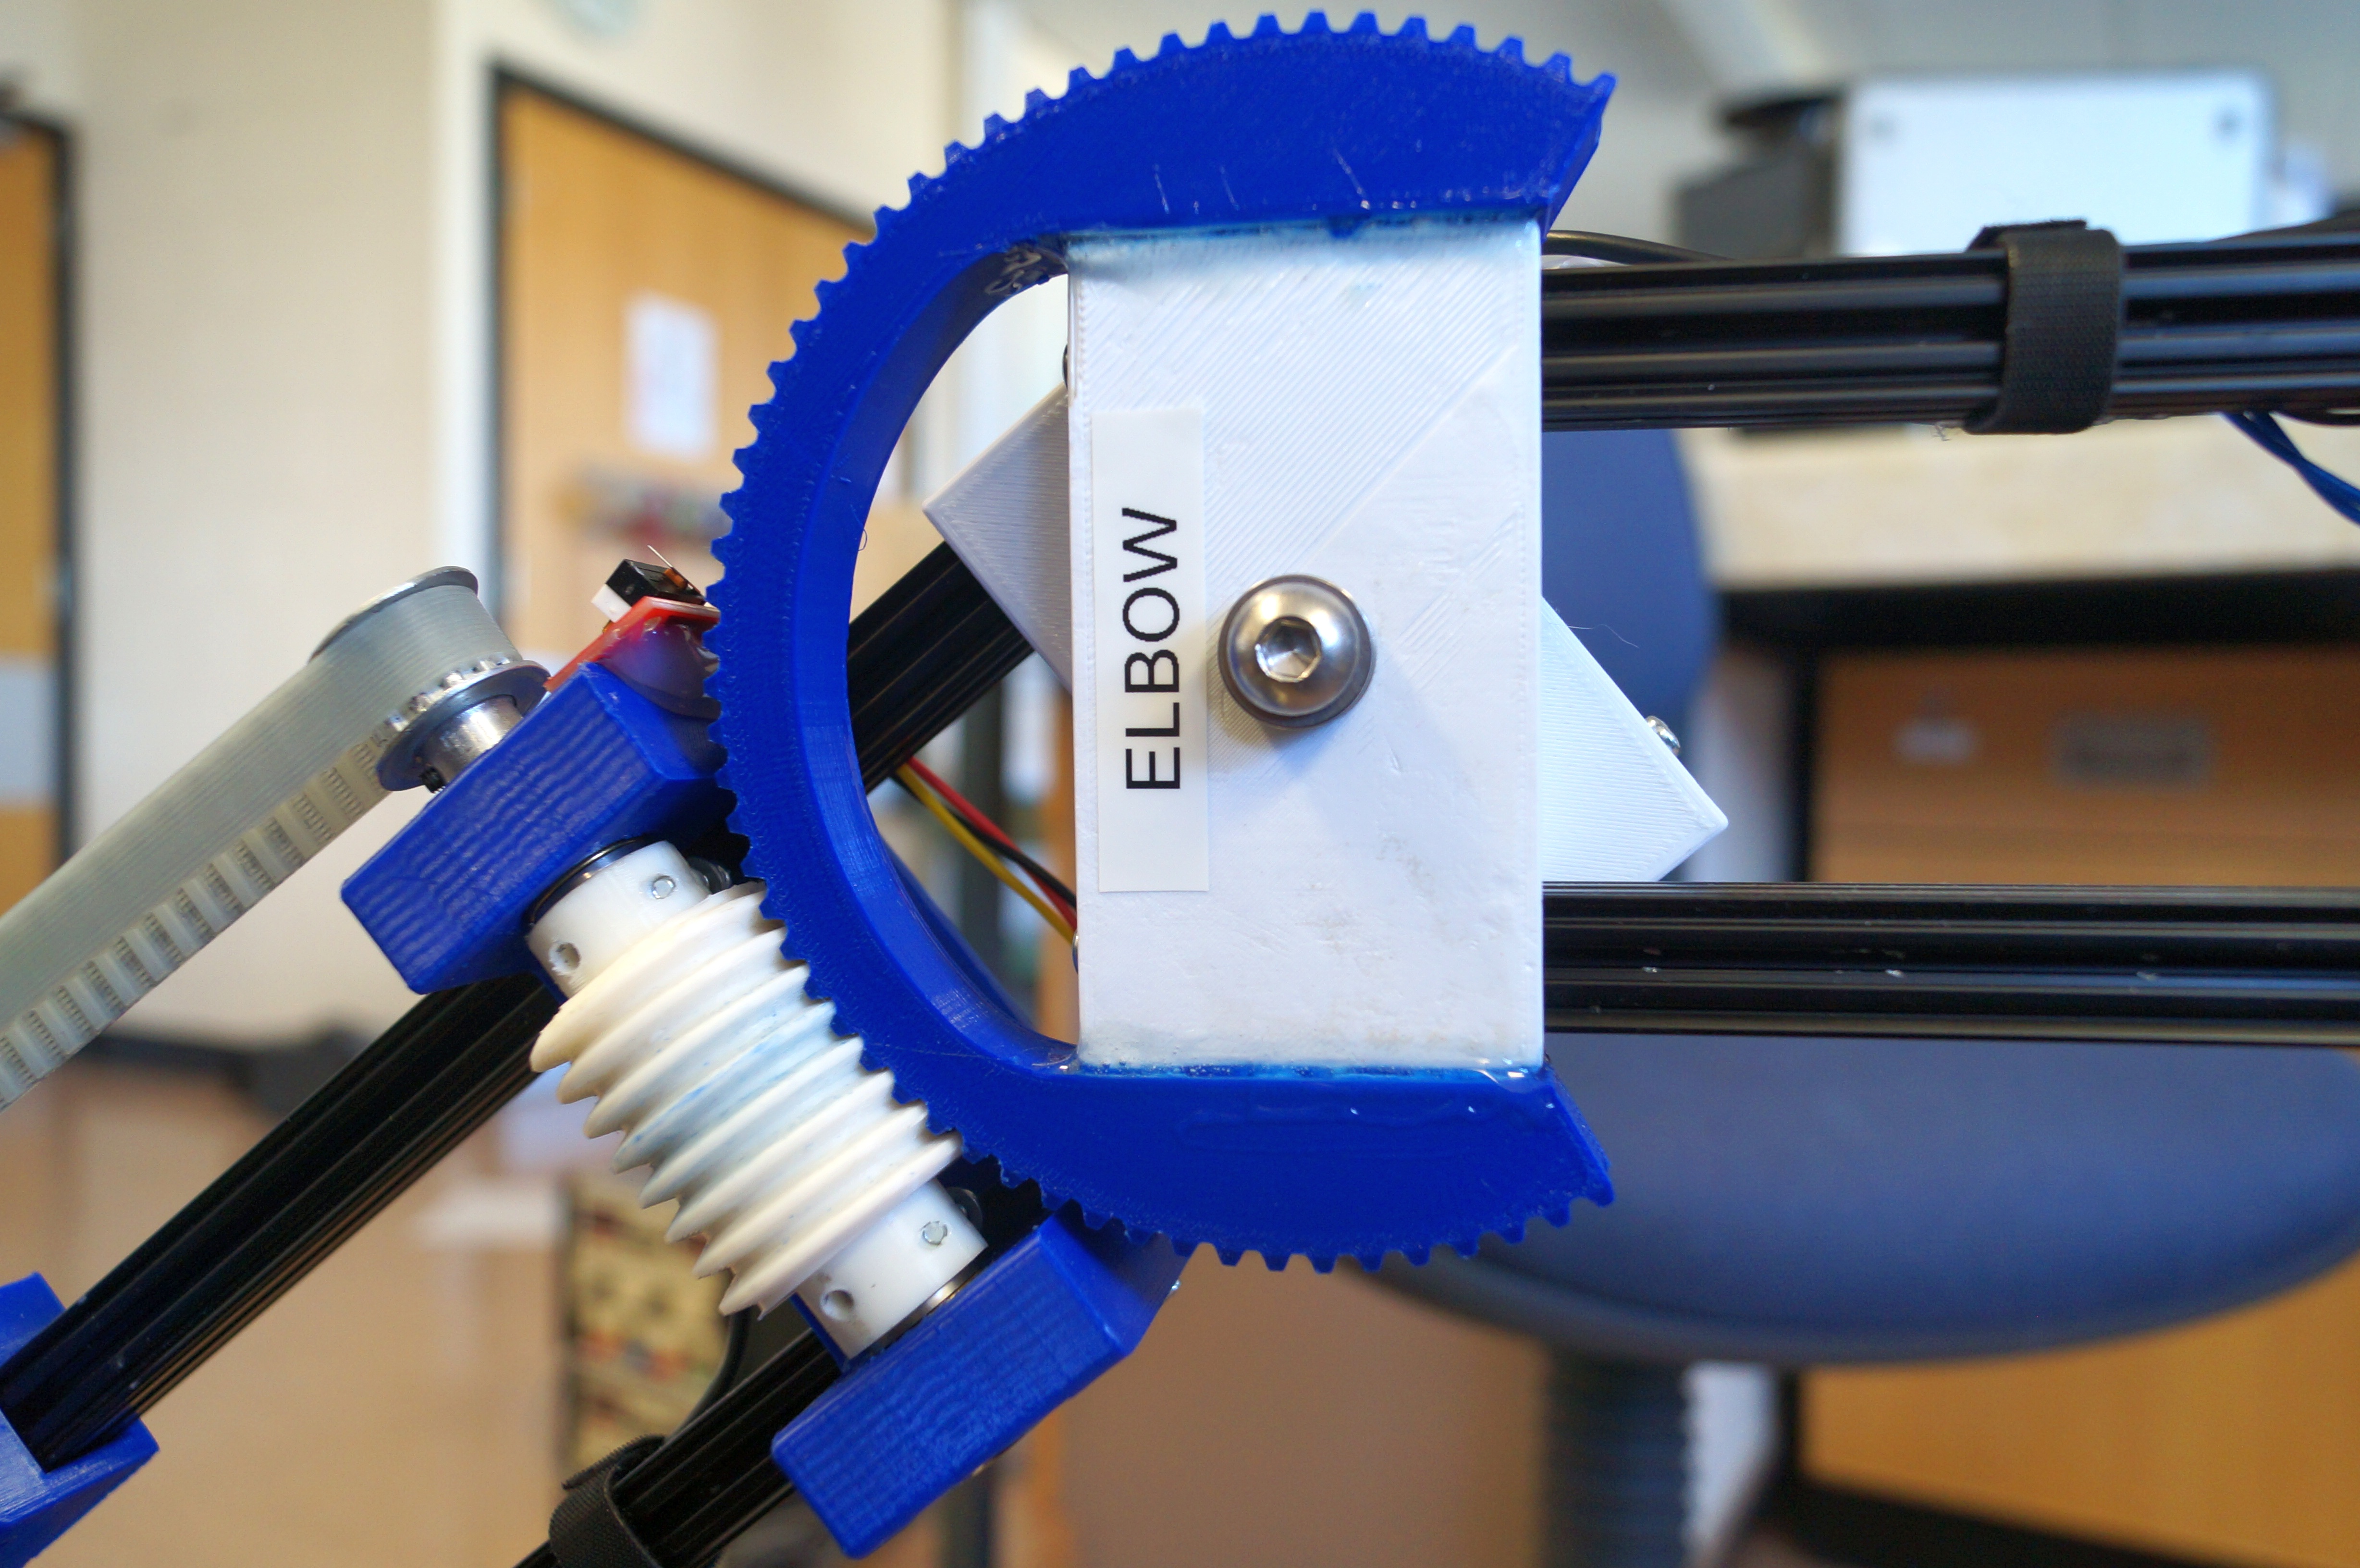
\includegraphics[width=10cm]{elbow.jpg}
\end{center}
\caption{Elbow Joint}
\label{fig:elbow}
\end{figure}

\subsubsection{Wrist}
The wrist is designed to always point down with another 4 bearings used to reduce friction. The joint block can be removed from the end of the arm easily by removing the M3 bolts that attach it to the end of the extrusion. This will facilitate extending the arm or changing the gripper.

\begin{figure}[!htb]
\begin{center}
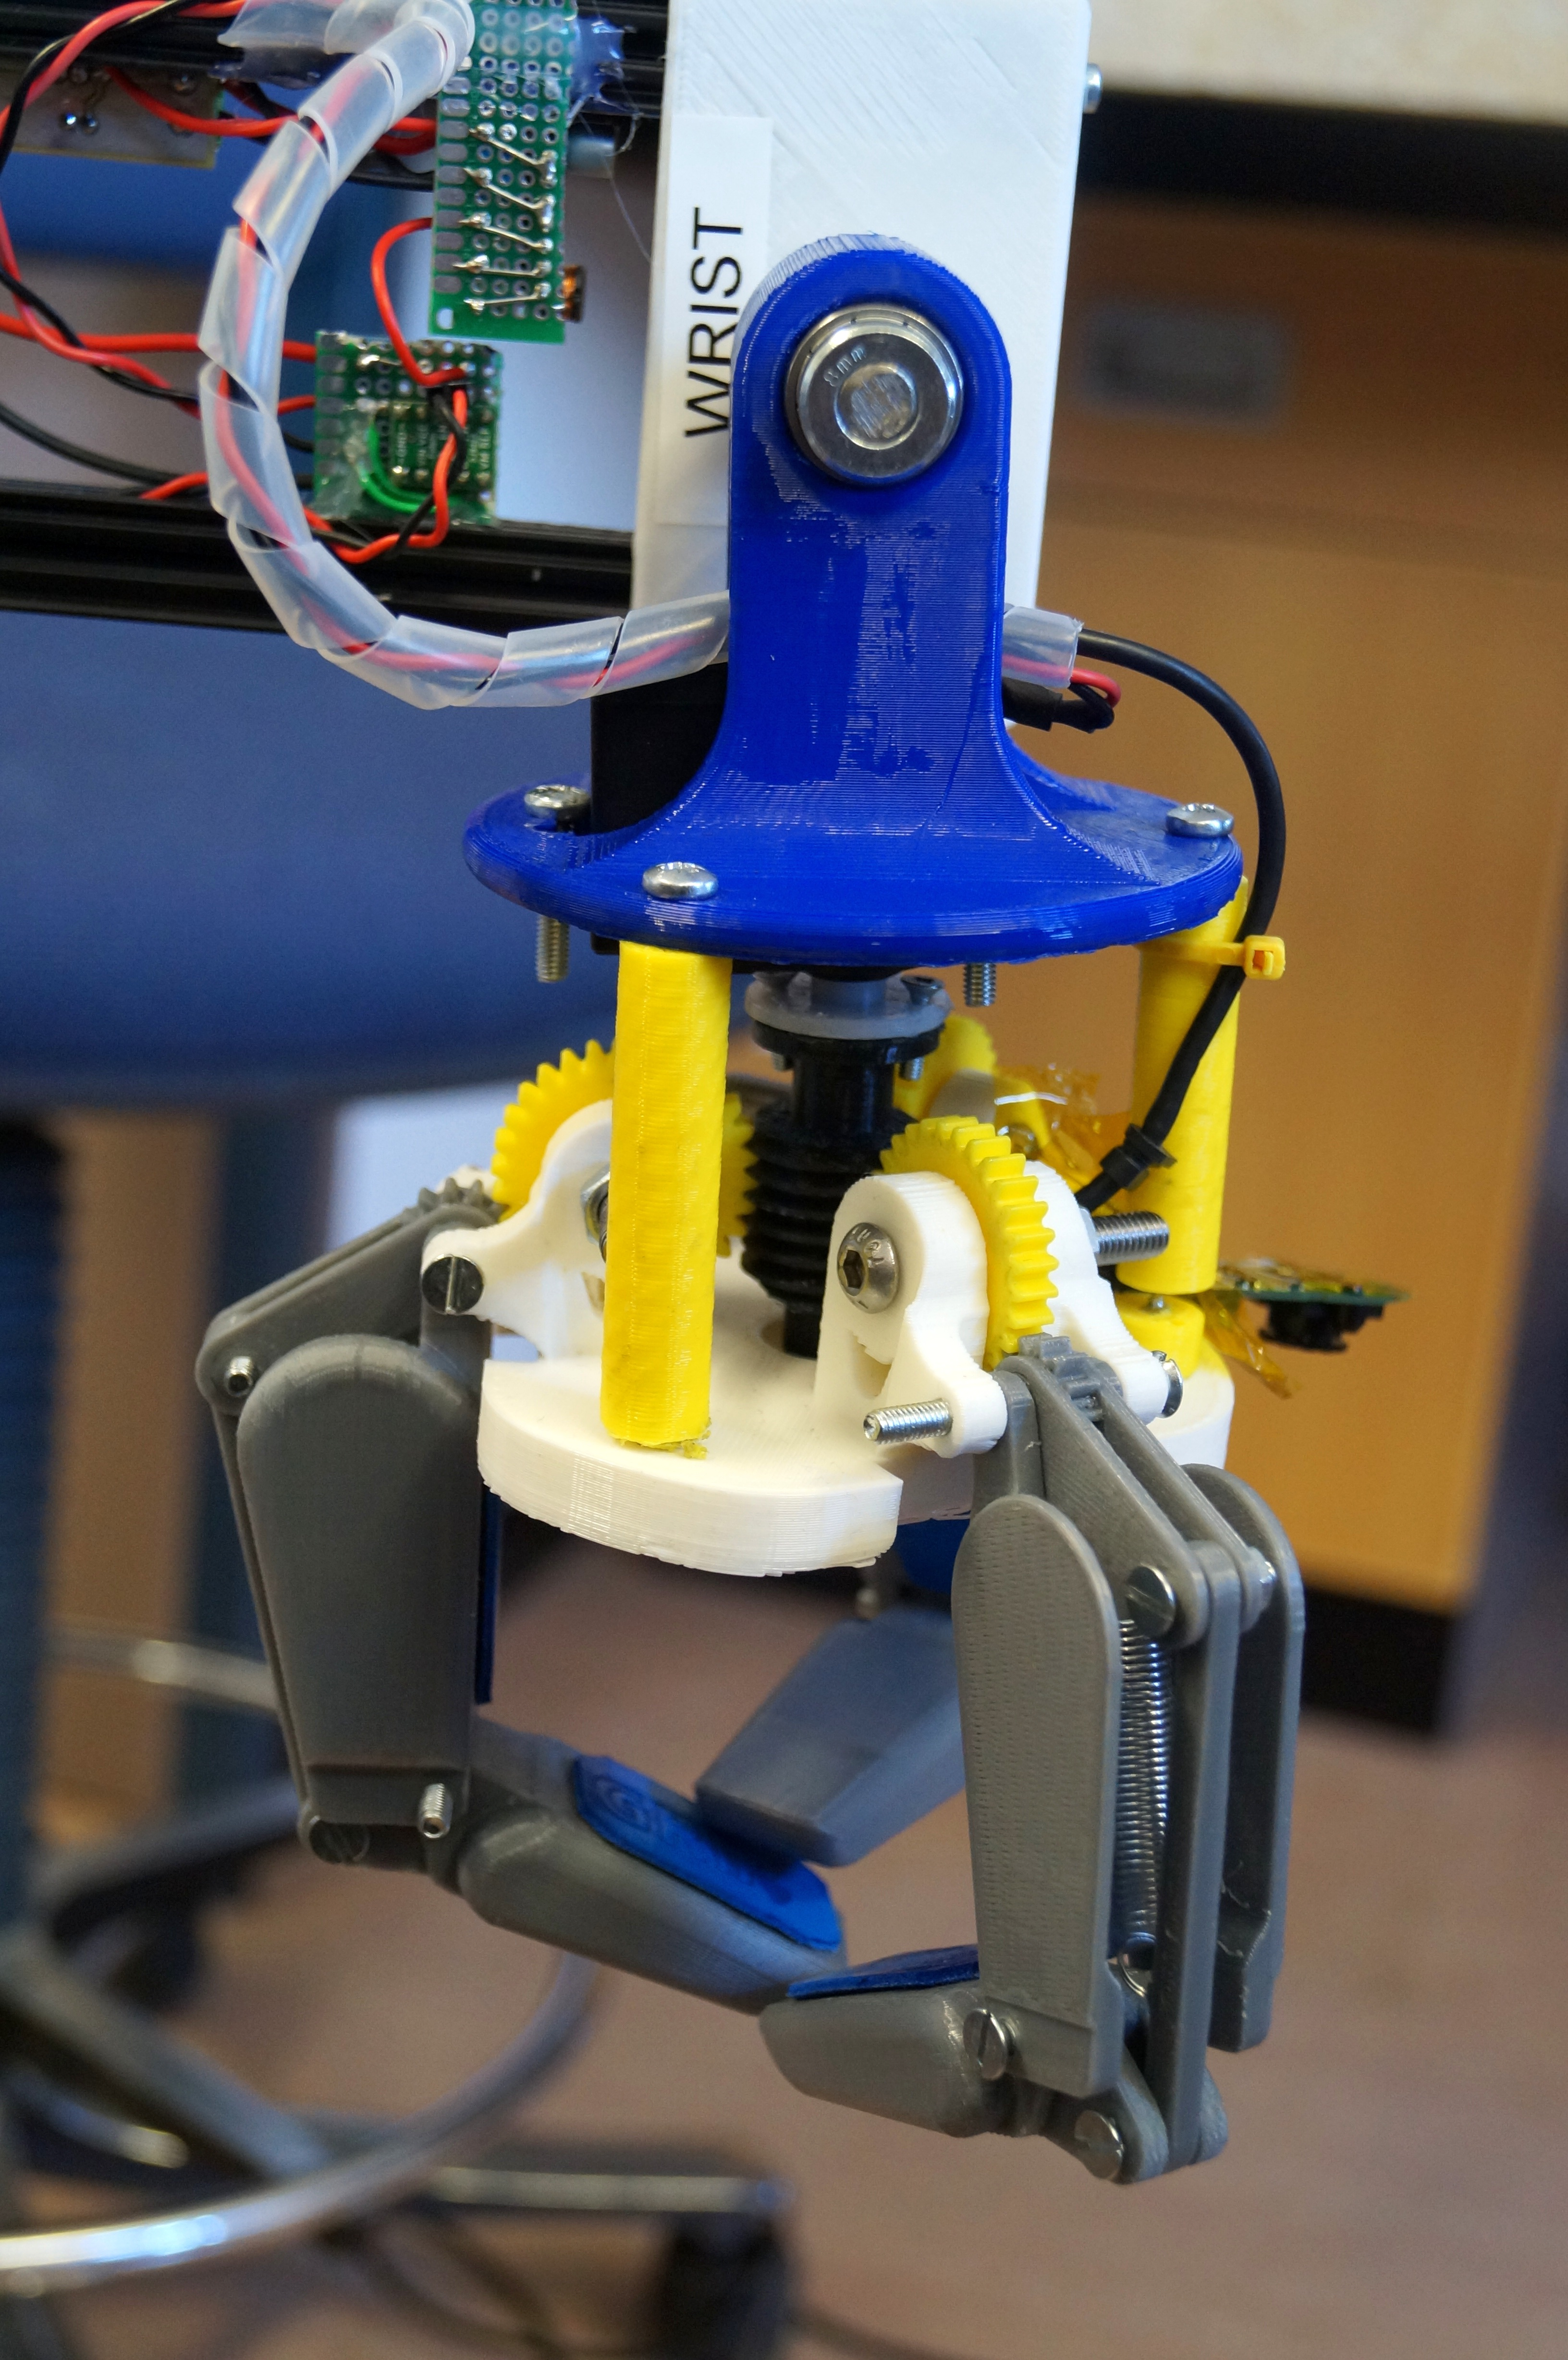
\includegraphics[width=10cm]{gripper.jpg}
\end{center}
\caption{Wrist Joint}
\label{fig:wrist}
\end{figure}

\subsubsection{End Effector}
The end effector was powered by a HITEC HS-5645MG servo modified for continuous rotation. The servo turns a worm gear which moves the fingers. The gripper has 5 states which give enough precision to pick up most objects. It also has a small USB webcam mounted on the side for teleoperation.


\subsubsection{Electronics}
An Arduino Mega 2560 with a RAMPS1.4 shield was used to control the arm. A modified version of Marlin (3d printer firmware) was used. This handled homing and moving to positions in joint space. Python code was written to interface with the firmware using G-Code  (RS-274 numerical control programming language) 

\subsubsection{Materials}
The arm was constructed using several different materials. The main load bearing beams use openbeam aluminium extrusion. PLA was used for all printed parts except the worm gear in the gripper which was printed in nylon 6.

\subsubsection{Parking} \label{parking}
The arm was designed to pick up objects and then put them into a basket and return to the park position so that Tiberius could continue on its mission unimpeded. This was chosen to be at an acute angle close to the back right wheel.

\subsubsection{Homing}
As discussed in \textit{Parking} \ref{parking} the arm will always start from the same location. This makes the task of homing relatively easy since we know where the arm will start. It was decided that the arm should home backwards which meant it would flip to a position at the front of Tiberius. The arm then moves to its centre location in front of Tiberius. 



\subsection{Software Design}
The main control code of the arm is designed to stop it from damaging itself or Tiberius. With allowed angles for each joint and position in Cartesian space defined. Assuming that the arm thinks it is in the correct location.

\subsubsection{Inverse Kinematics}

This involved taking a 3 dimensional Cartesian coordinate and converting it into angular coordinates that the three arm joints would position to.  The basic way this was done was by using trigonometry to identify the required rotation angle, which would be done with the waist joint and by using further trigonometry to determine the two joint angles required to manoeuvre the joints to the correct point in space.	
\newline
The code was designed to be flexible and adaptable so the arm segments’ lengths were used as parameters in the code along with the x, y and z Cartesian coordinates of the desired position.  
\newline
Each Cartesian coordinate was converted into the angles of the three motors from rest, which were denoted as $\rho$, $\sigma$ and $\tau$.  The angle of rotation, $\rho$ around the base of the arm, was controlled by a large stepper motor, $\tau$ was the angle of the upper arm joint which could be positioned forwards or backwards depending on the depth of the object being picked up and $\sigma$ was the angle of the elbow joint which allowed the gripper to be positioned above the object of interest.  

\begin{figure}[!htb]
\begin{center}
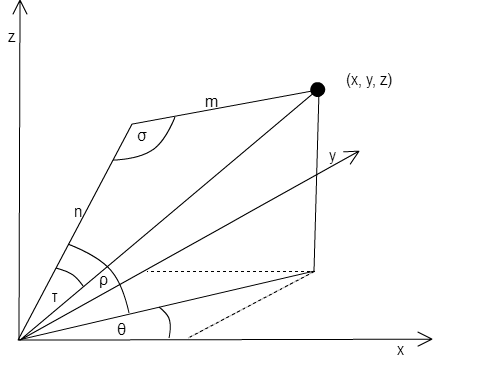
\includegraphics[width=15cm]{Cartesian2.png}
\end{center}
\caption{Transformation from Cartesian Coordinates}
\label{fig:cartesian}
\end{figure}

\begin{capequ}[!htb]
\begin{center}
\begin{equation}
\theta = tan^{-1}\left (  \frac{y}{x}\right )
\end{equation}
\caption{Rotation Angle of Base}
\label{Equation4}
\end{center}
\end{capequ}

The first angle to be calculated is the azimuthal angle which is the horizontal plane angle, which is controlled by the base motor.
This angle can be calculated by using the inverse tangent function of the y and x coordinate

\begin{capequ}[!htb]
\begin{center}
\begin{equation}
\tau = cos^{-1}\left (\frac{m^{2}+s^{2}-n^{2}}{2ms}\right )
\end{equation}
\caption{Acute angle from the triangle facing the object}
\label{Equation6}
\end{center}
\end{capequ}

\begin{capequ}[!htb]
\begin{center}
\begin{equation}
\rho = tan^{-1}\left ( \frac{z}{\sqrt{{x^{2}+y^{2}}}} \right )+ cos^{-1}\left ( \frac{m^{2}+(x^{2}+y^{2}+z^{2})}{2mn} \right )
\end{equation}
\caption{Elevation Angle of Upper Arm}
\label{Equation3}
\end{center}
\end{capequ}


\begin{capequ}[!htb]
\begin{center}
\begin{equation}
\sigma = cos^{-1}\left (\frac{m^{2}+s^{2}-(x^{2}+y^{2}+z^{2})}{2ms} \right )
\end{equation}
\caption{Elbow Joint Angle}
\label{Equation5}
\end{center}
\end{capequ}

The remaining angles were calculated using some more advanced trigonometry and these were finally passed to the motor controllers.  This was all implemented in Python which uses simple functions such as acos, atan etc.


\subsubsection{Safety}
Since the arm is easily capable of damaging itself due to the very high torque outputs it was necessary to write the code in a way that never allowed commands to be run out of order. For example it should not be possible to move the arm until it has been homed and put the the centre position since at this point it can be limited to an area in front of Tiberius. The code also stops any command that would lead to a joint angle that is out of the arms range of motion.

\subsubsection{Manual Control}
The arm can be manually controlled either from the web interface or using the full control script. At the time of writing the web interface can only operate using joint rotations and the full control script has full functionality implemented.

\subsubsection{Camera}
The gripper has a small web cam attached so the user can see what is being picked up. This enables remote control of the arm through the web interface in real time.
